
\section{Timeline Simulation and Scenario Selection}
\todo{eventuel scenario selection nochmal abspalten als extra subsubsection}
\textbf{wie werden die verschiedenen Zeitreihen erzeugt}\\
Um auf gute allgemeine Strategien schließen zu können braucht es gute Daten. Falsche daten würden auch zu falschen Ergebnissen/Strategien führen.
Dabei gibt es verschiedene Ansätze diese Zeitreihendaten zu erstellen. Es folgt zuerst ein Überblick über die realwelt Daten um einen besseren eindruck
davon zu bekommen was wir probieren nach zu armen / vorherzusagen bzw. über welche wesentlichen eigenschaften die verschiedenen Marktdaten verfügen
Dazu werden die verschiedenen Marktdaten statischtisch dargestellt.
Anschließend werden verschiedene Analysemethoden diskutiert, kombiniert und angewandt.
In diesem Abschnitt werden verschiedene Methoden zur Erstellung von Zeitreihen diskutiert.
\subsubsection{Market Data Analysis}
\textbf{RL}\\
Im ersten Fenster der übersicht [\ref{fig:Overview Average Negativ Capacity Price}] sind der Realmarktdaten von 2023 für den negativen Kapazitätsmarktpreis zu sehen.
Darunter ist der Trend und die Saisonalität abgebildtet.

\begin{figure}[!h]
	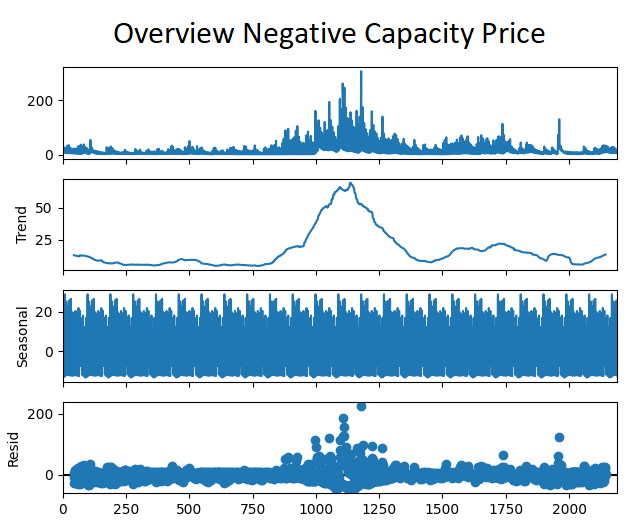
\includegraphics[width=0.7\linewidth]{pictures/capacityData_overview.png}
	\caption{Total Average Negativ Capacity Price}
	\label{fig:Overview Average Negativ Capacity Price}
\end{figure}

Bei einer genaueren Untersuchung der Saisonalität zeigt siche ein täglicher und ein leichter Wöchentlicher rythmus in den Daten.
Da es sich um Daten handelt die sich auf 4h-Blöcke beziehen sind alle 6 Lags als ein Tag zu interpretieren.
Abbildung \ref{fig:Autocorrelation Negative Capacity Price - 5 Days} zeigt dabei eine klaren täglichen rythmus in den Daten.

\todo{price in titel ergänzen}
\begin{figure}[!h]
	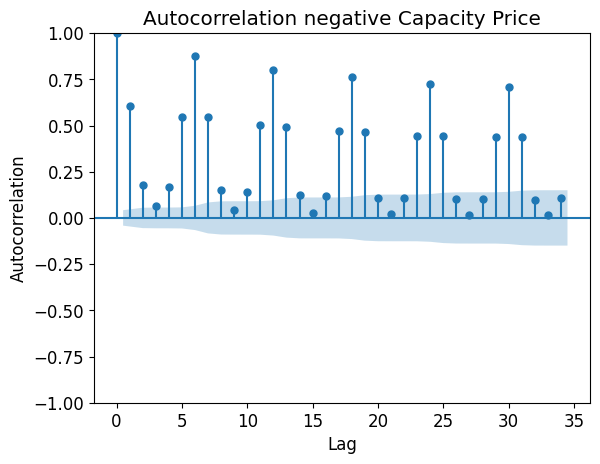
\includegraphics[width=0.7\linewidth]{pictures/Autocorrelation negative Capacity Price.png}
	\caption{Autocorrelation Negative Capacity Price - 5 Days}
	\label{fig:Autocorrelation Negative Capacity Price - 5 Days}
\end{figure}

Und Abbildung \ref{fig:AutocorrNegCap4Weeks} lässt zudem einen leichten wöchentlichen Zyklus erkennen.
\begin{figure}[!h]
	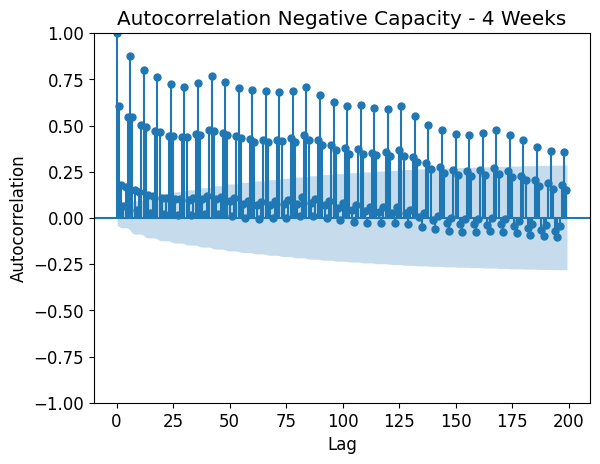
\includegraphics[width=0.7\linewidth]{pictures/Autocorrelation Negative Capacity - 4 Weeks.png}
	\caption{Autocorrelation Negative Capacity Price - 4 Weeks}
	\label{fig:AutocorrNegCap4Weeks}
\end{figure}

Die Preise zu den positiven Kapazitätwerten verhalten sich ähnlich wie die negativen Kapazitätswerte.

Zur anaylse und Zeitreihenvorhersage dieser Daten bieten sich nun, aufgrund der starken autocorrelation verschiedene statistische methoden an.
Dabei stellt sich besonders die ARIMA methode heraus. Diese beruht auf autoregression und ist somit besonders gut für zeitreihen mit starker
autorkorrelation geeignet. Um auch die Saisonalen effekte gut abbilden zu können gibt es eine Variante the ARIMA methode die SARIMA methode.

Ein ausführlicher Test der SARIMA methode, und der dafür notwendigen Tests befindet sich in Appendix \todo{verweis einfügen}. Dabei hat sich gezeigt, das die SARIMA methode schwächen mit der
komplexität in sehr langen Zeitreihen hat. So stieg die Rechenzeit expotential an und langfriste vorhersagen zeigten eine klare verzerrung hinsichtlich des letzten Trends.
Da wir aber kurzfristig ähnliche Jahresverläufe erwarten ist diese verzerrung folgend dem Trend am Jahresende nicht sinnvoll.
Außerdem ist die SARIMA analyse dafür ausgelegt Zeitreihendaten mit nur einer saisonalität zu erstellen. Für multiple Saisonalitäten wären aufwendige
manuelle anpassungen nötig. Ein Algorithmus der diese Nachteile vermeidet fußt auf den vorher genannten Konzepten und nennt sich TBATS.
TBATS is acronym for Trigonometric seasonality Box-Cox transformation ARMA errors Trend Seasonal components. Dieser Algorithmus von SKTIME erlaubt eine
einfachere Zeitreihenvorhersage bei gegebener multipler Saisonalität \cite{.05.04.2025}. \todo{appendix verweis}

Die somit vorhergsagte Zeitreihe ähnelt sehr der realen Zeitreihe [Abbildung \ref{fig:Negative Capacity Price Prediction - 2023}]. zu Beachten ist das die hier zu sehende Zeitreihe die Zeitreihe mit der höchsten Wahrscheinlichkeit ist.
So liegen 50\% der möglichen betrachteten Werte darüber und 50\% darunter. Wenn wir mit hilfe des vortrainierten predictors mehrere Szenarien/Zeitreihen
erstellen wollen so führt die inherente steigende ungewissheit mit steigenden Zeitabstand zu einer größerem intervall in dem die Daten liegen [Abbildung \ref{fig:Negative Capacity Price Prediction Interval - 2023}].
Das macht inhaltlich sinn und mag für viele anwendungsfälle sinnvoll sein, wir gehen aber davon aus das die mittlere vorhersage nicht an genauigkeit verliert
und wollen daraus szenarien generieren. Zu diesem Zweck wird die wahrscheinlichste/mittlere zeitreihenvorhersage genommen und manuel nach oben und nach unten
um bestimmte Prozentsäte hoch bzw. herunterskaliert. Die so erstellten Preisvorhersagen werden dann mit den realen Preisen verglichen und berechnet zu wievielen
Prozent mit der skalierten Zeitreihe ein Gebotszuschlag erfolgt wäre.

\begin{figure}[!h]
	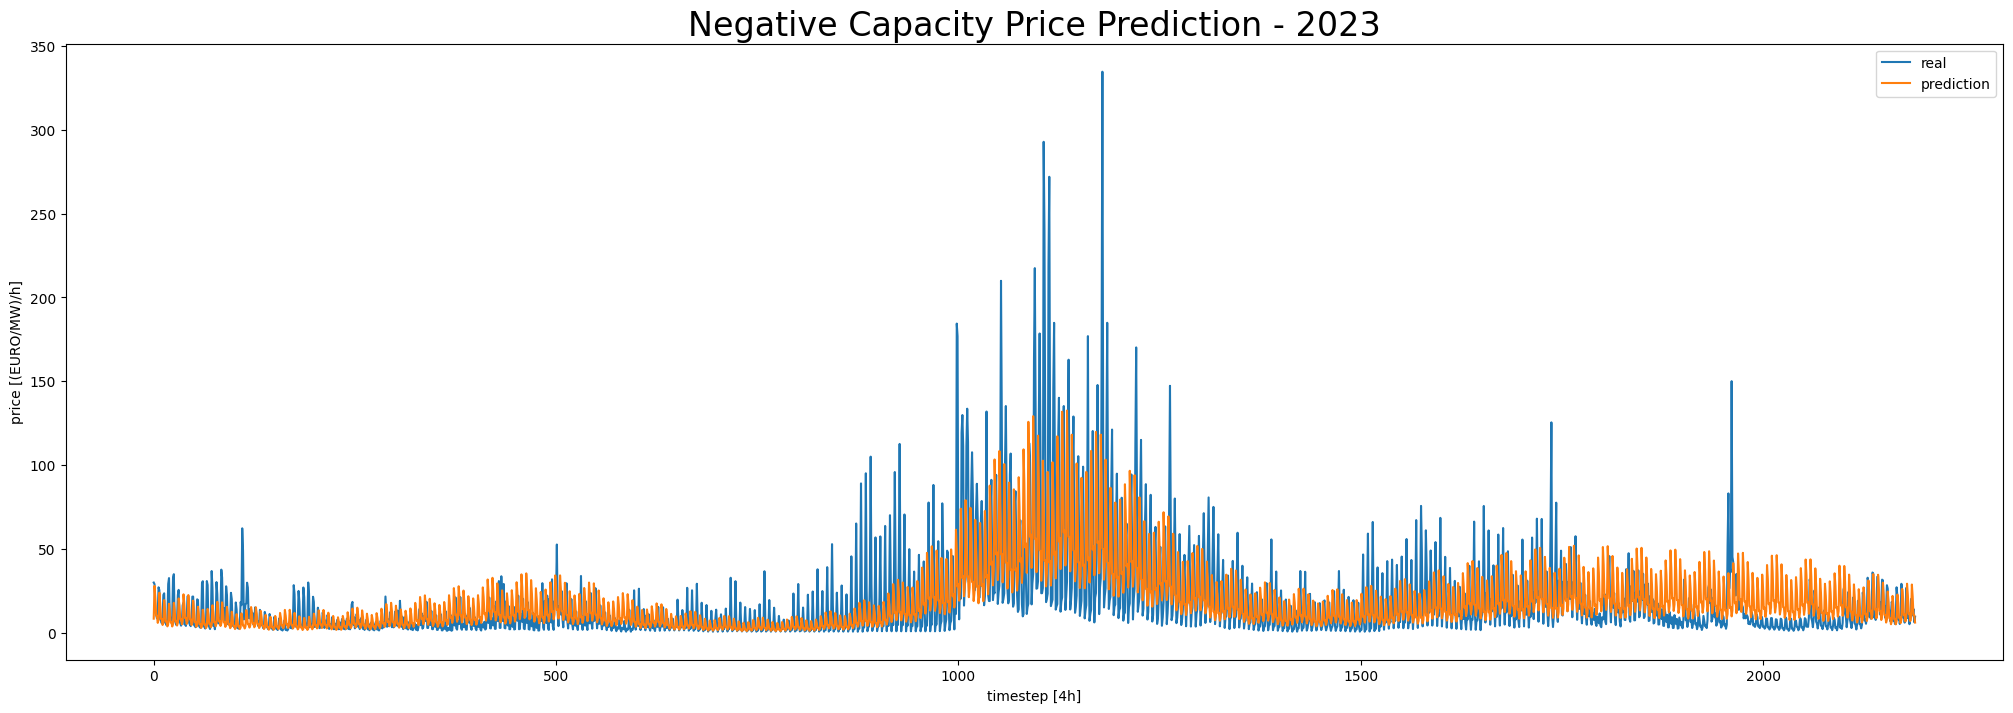
\includegraphics[width=1\linewidth]{pictures/RL/Negative Capacity Price Prediction - 2023.png}
	\caption{Negative Capacity Price Prediction - 2023}
	\label{fig:Negative Capacity Price Prediction - 2023}
\end{figure}

\begin{figure}[H]
	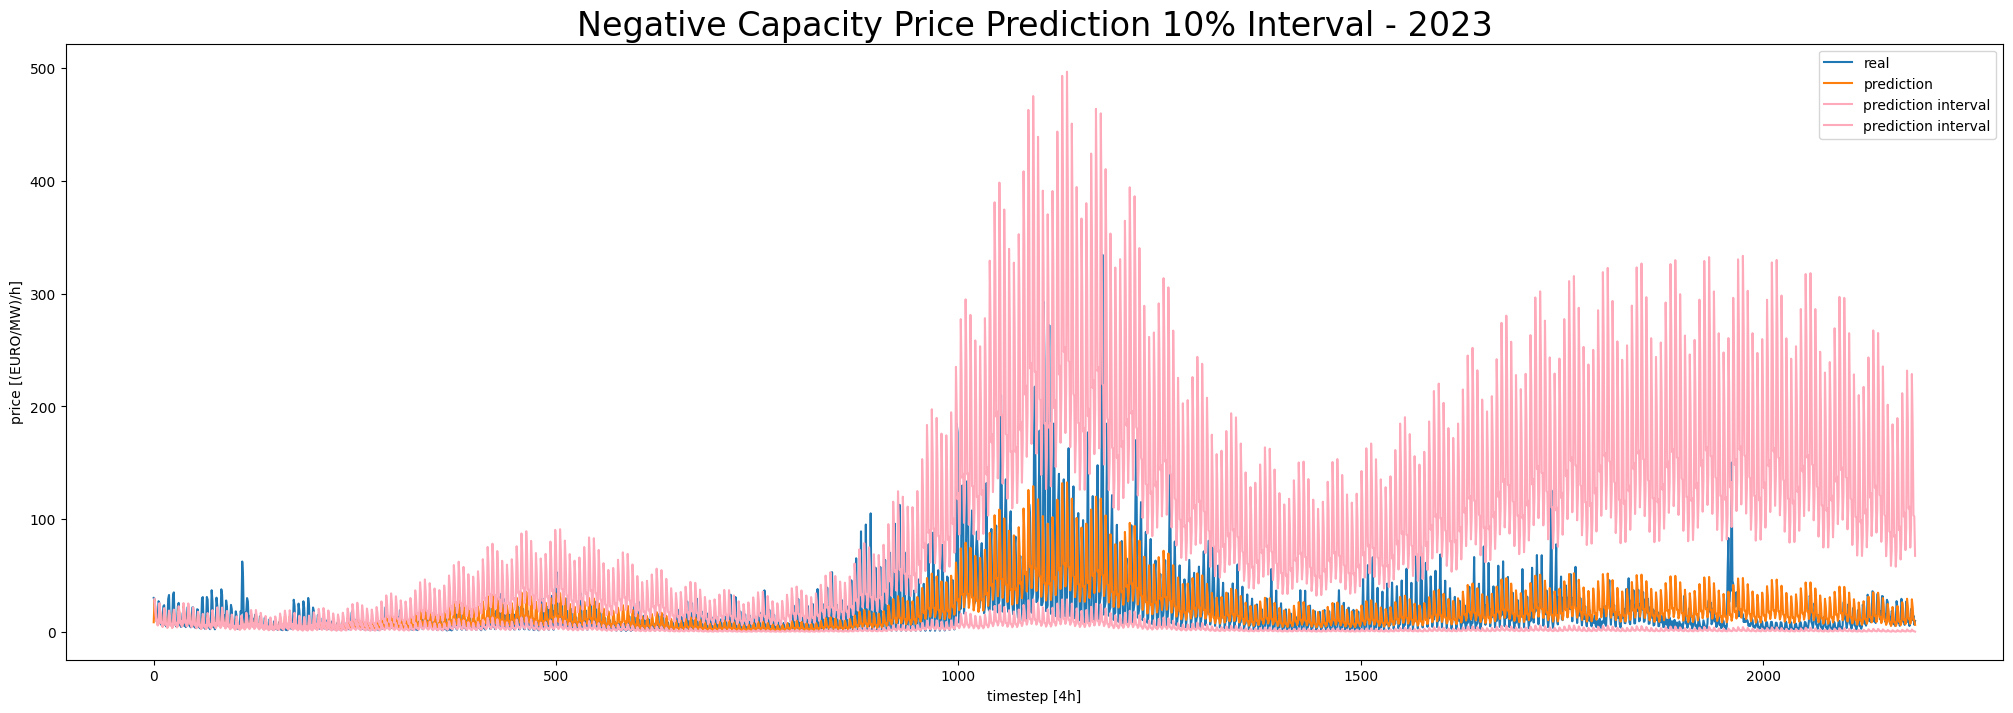
\includegraphics[width=1\linewidth]{pictures/RL/Negative Capacity Price Prediction Interval - 2023.png}
	\caption{Negative Capacity Price Prediction 10\% Interval - 2023}
	\label{fig:Negative Capacity Price Prediction Interval - 2023}
\end{figure}

- hier eventuell noch rein das wenige daten ein hohes rauschen erzeugen
- wobei zuviele daten ein overfitting verursachen können



\textbf{DA}\\
Die Day-Ahead Markt Preise sind zwar Variabel unterliegen aber einem Täglichem wie Wöchentlichen Rythmus.
Im Jahresverlauf sind nur allgemeine Trends ablesbar wie Abbildung \ref{fig:overviewDAprices} zeigt.
\begin{figure}[!h]
	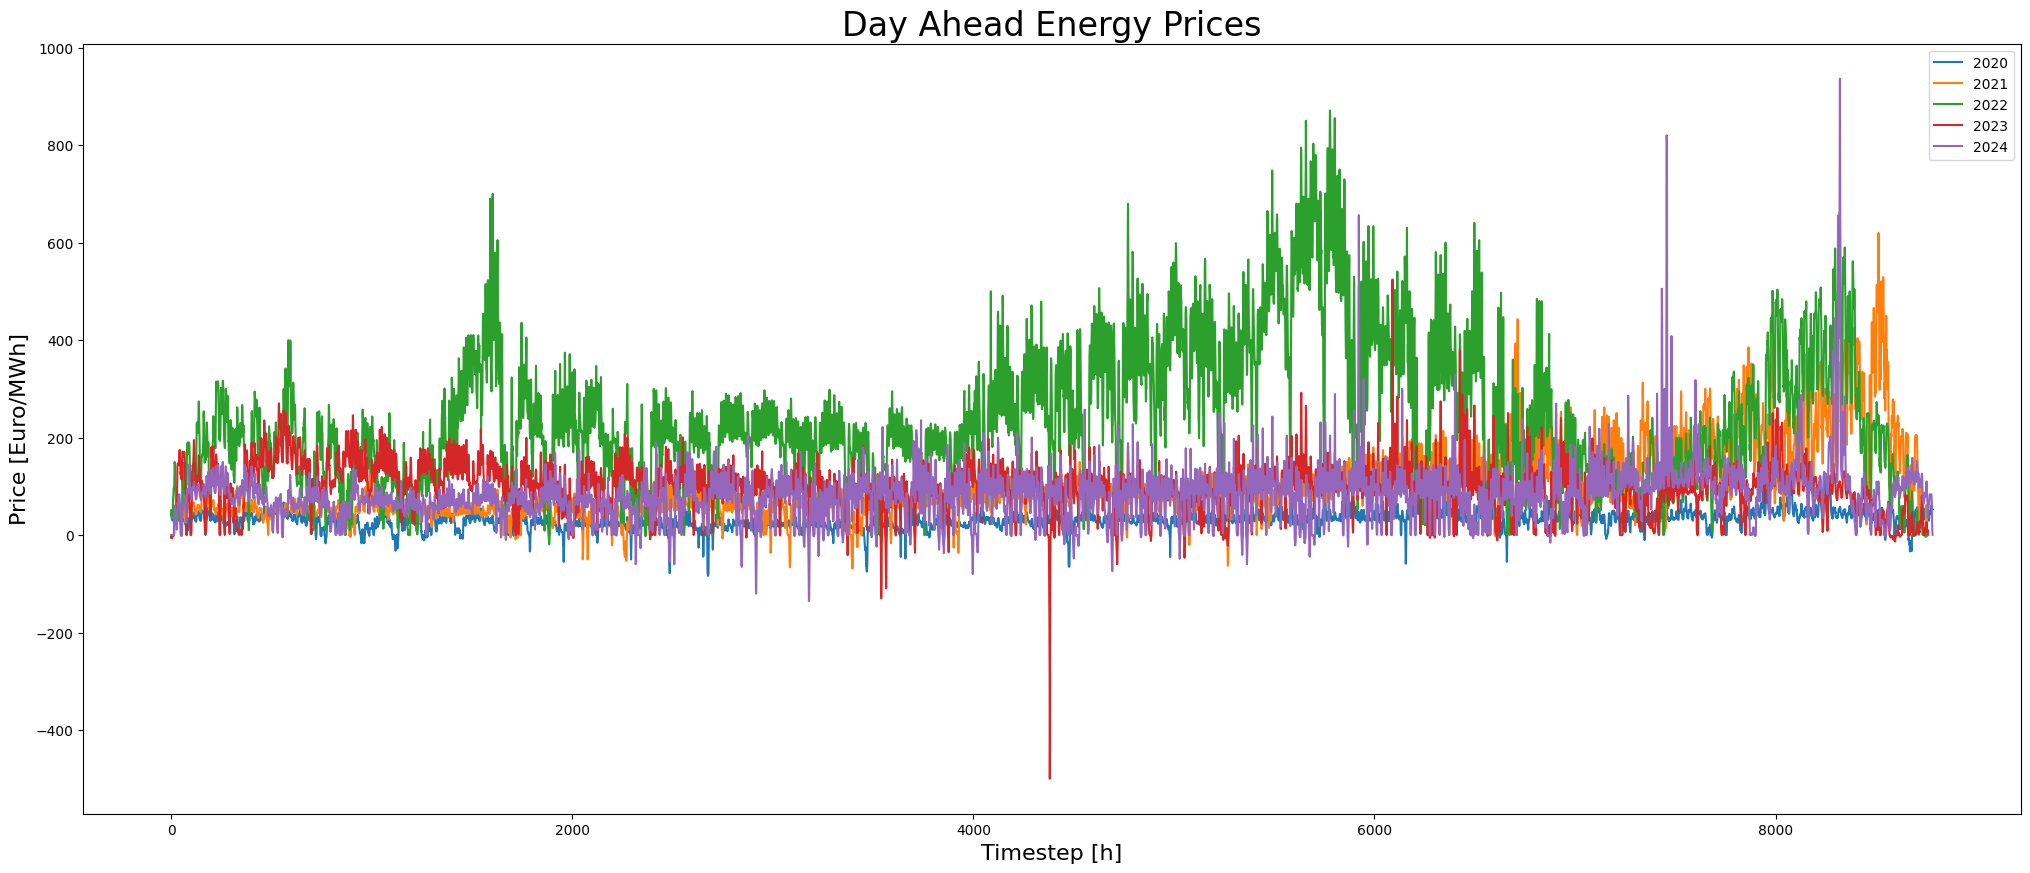
\includegraphics[width=1\linewidth]{pictures/overviewDAprices_year.png}
	\caption{Overview DA prices}
	\label{fig:overviewDAprices}
\end{figure}
Die außergewöhnliche Kurvenbewegung im Jahr 2022 ist mit dem Angriffskrieg Russlands gegen die Ukraine zu erklären
und den daraus folgenden Turbulenzen am Gas Markt.

Da es sich beim DA Markt um einen pay-as-cleared markt handelt (alle bekommen den Preis des am höchsten bezugschlagtem Teilnehmers)
und wir als Produzent erneurbarer Energien mit sehr geringen Opperationalen Kosten zu tun haben ist es für das model nur wichtig ob
wir am markt teilnehmen und welcher clearing price zu erwarten ist.

wie and Grafik \ref{fig:meanDA2020} bis \ref{fig:stdDA2024}      zu entnehmen ist zeigt der clearing price einen täglichen und wöchentlich  rythmus.
Das Nivau verändert sich zwar lässt sich aber gut verhersagen. Aufgrund des Marktdesigns brauchen wir auch nur einen erwarteten clearing price
da wir in der Realität ein 0-Preis Gebot abgeben können und somit sogut wie sicher bezuschlagt werden.
Der Erwartete Preis wird für unser Model als Mittelwert der Jahre 2020 bis 2024 ohne das Jahr 2022 kalkuliert. So erhalten die
Saisonale Struktur in den Daten und gleichen Ausreißer nach oben sowie nach unten aus. So ergibt sich je nach Tageszeit, Wochentag und Jahresverlauf ein zuverlässig
zu erwartender clearing-price. Das Nivau kann auch noch nachträglich leicht durch einen Skalierungsfaktor angepasst werden ohne die inherente Struktur der Daten zu gefährden.

\begin{figure}[H]
	\centering
	\begin{minipage}{0.49\textwidth}
		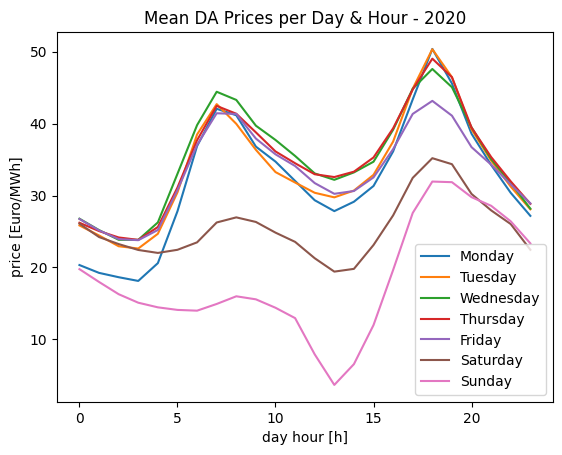
\includegraphics[width=1\linewidth]{pictures/DA/Mean DA Prices per Day and Hour - 2020.png}
		\subcaption{Mean DA-Price}
		\label{fig:meanDA2020}
	\end{minipage} \hfill
	\begin{minipage}{0.49\textwidth}
		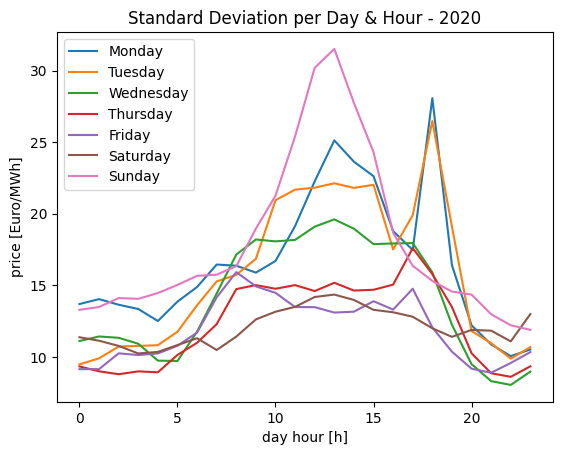
\includegraphics[width=1\linewidth]{pictures/DA/Standard Deviation per Day and Hour - 2020.png}
		\subcaption{Standard Deviation DA-Price}
		\label{fig:stdDA2020}
	\end{minipage}
	\caption{Daily and hourly DA-Data - 2020 }
\end{figure}

\begin{figure}[H]
	\centering
	\begin{minipage}{0.49\textwidth}
		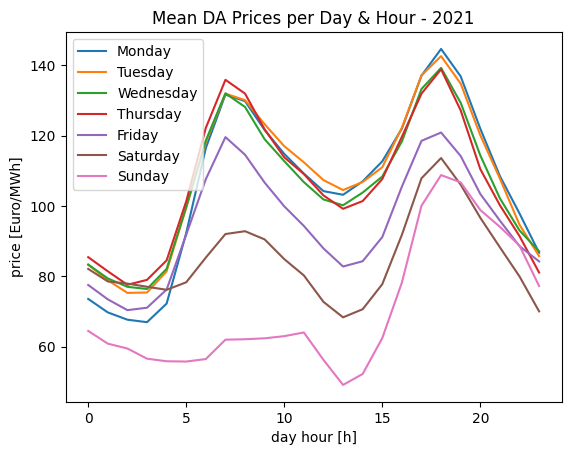
\includegraphics[width=1\linewidth]{pictures/DA/Mean DA Prices per Day and Hour - 2021.png}
		\subcaption{Mean DA-Price }
		\label{fig:meanDA2021}
	\end{minipage} \hfill
	\begin{minipage}{0.49\textwidth}
		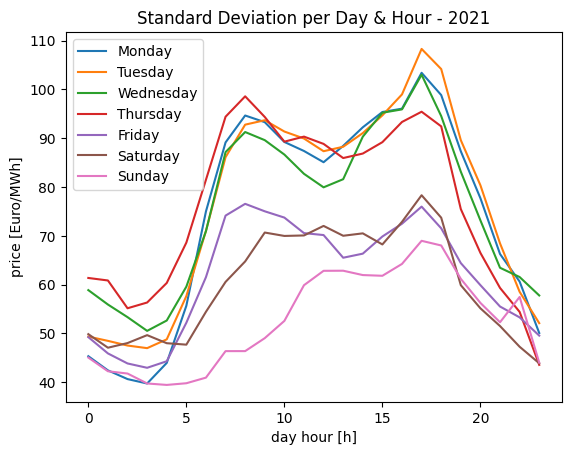
\includegraphics[width=1\linewidth]{pictures/DA/Standard Deviation per Day and Hour - 2021.png}
		\subcaption{Standard Deviation DA-Price}
		\label{fig:stdDA2021}
	\end{minipage}
	\caption{Daily and hourly DA-Data - 2021 }
\end{figure}

\begin{figure}[H]
	\centering
	\begin{minipage}{0.49\textwidth}
		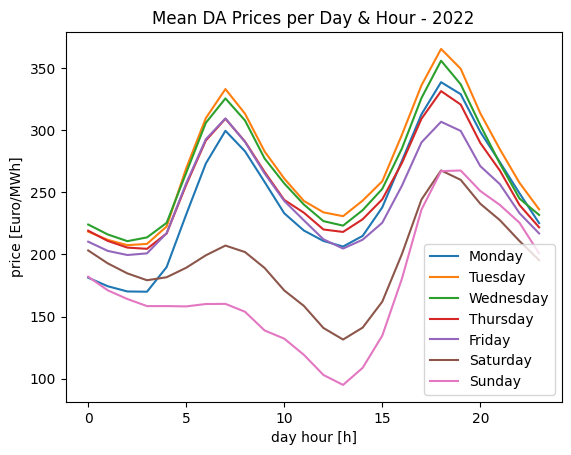
\includegraphics[width=1\linewidth]{pictures/DA/Mean DA Prices per Day and Hour - 2022.png}
		\subcaption{Mean DA-Price }
		\label{fig:meanDA2022}
	\end{minipage} \hfill
	\begin{minipage}{0.49\textwidth}
		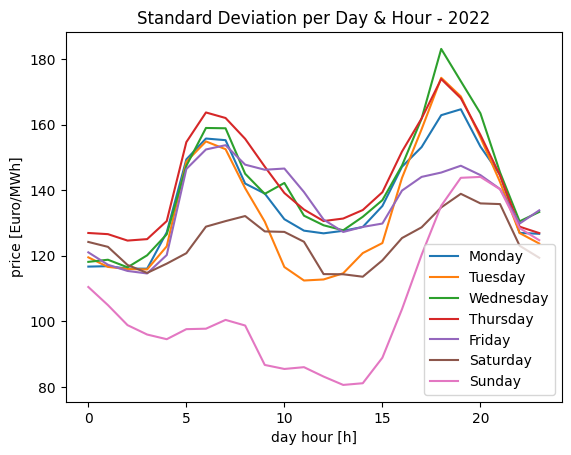
\includegraphics[width=1\linewidth]{pictures/DA/Standard Deviation per Day and Hour - 2022.png}
		\subcaption{Standard Deviation DA-Price}
		\label{fig:stdDA2022}
	\end{minipage}
	\caption{Daily and hourly DA-Data - 2022 }
\end{figure}

\begin{figure}[H]
	\centering
	\begin{minipage}{0.49\textwidth}
		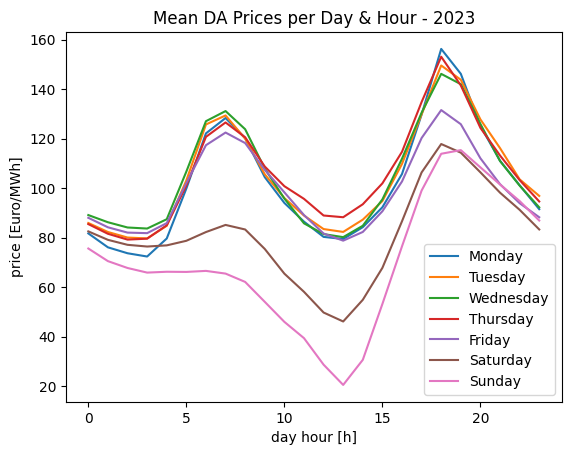
\includegraphics[width=1\linewidth]{pictures/DA/Mean DA Prices per Day and Hour - 2023.png}
		\subcaption{Mean DA-Price }
		\label{fig:meanDA2023}
	\end{minipage} \hfill
	\begin{minipage}{0.49\textwidth}
		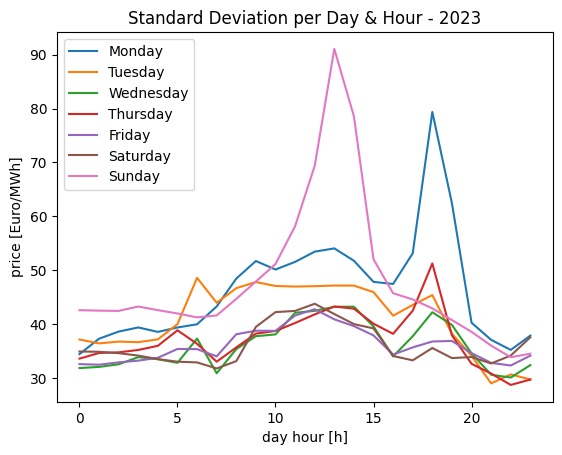
\includegraphics[width=1\linewidth]{pictures/DA/Standard Deviation per Day and Hour - 2023.png}
		\subcaption{Standard Deviation DA-Price}
		\label{fig:stdDA2023}
	\end{minipage}
	\caption{Daily and hourly DA-Data - 2023 }
\end{figure}

\begin{figure}[H]
	\centering
	\begin{minipage}{0.49\textwidth}
		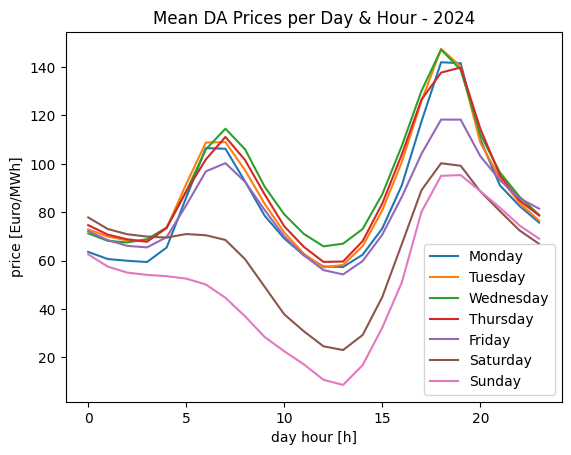
\includegraphics[width=1\linewidth]{pictures/DA/Mean DA Prices per Day and Hour - 2024.png}
		\subcaption{Mean DA-Price }
		\label{fig:meanDA2024}
	\end{minipage} \hfill
	\begin{minipage}{0.49\textwidth}
		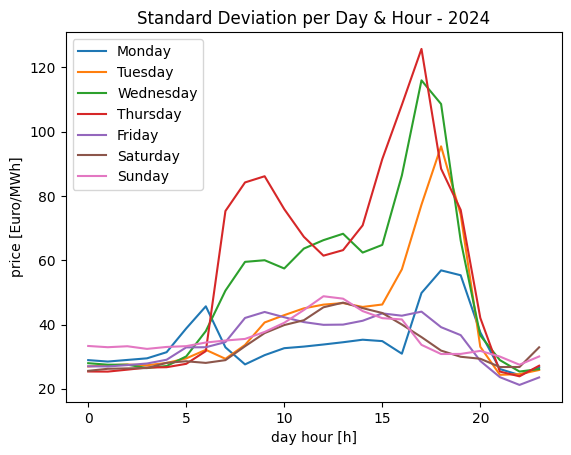
\includegraphics[width=1\linewidth]{pictures/DA/Standard Deviation per Day and Hour - 2024.png}
		\subcaption{Standard Deviation DA-Price}
		\label{fig:stdDA2024}
	\end{minipage}
	\caption{Daily and hourly DA-Data - 2024 }
\end{figure}

Des weiteren gehen wir für unsere Simulation davon aus das der simulierte erneuerbare Energien park ein onshore wind park in
Deutschland ist. Um ein Windprofil zu erhalten dividieren wir die gesamte produktion von onshore windanlagen durch die gesamte Kapazität dieser anlagen [\cite{.08.04.2025}].
Das gewonnene profil entspricht aber dem mittelwert der deutschen windonshore produktion. Sprich sie ist der mittelwert des
windes der über ganz deutschland weht. so arbeiten nie alle windkraftanlagen in deutschland gleichzeitig bei 100\%. das
kann aber für unseren einzelnen windpark durchaus passieren. Um der begrenzung der maximalen Anschlusskapazität also eine
sinnvolle bedeutung zu geben müssen wir also dieses profil entsprechend skalieren.
Hierfür gehen wir davon aus das die gesamte deutsche windproduktion zumindest ein indikator dafür ist wieviel wind gerade
an unserer anlage weht, skalieren aber die tiefen runter und die höhen hoch. eine weitere bedingung der neuberechnung ist
das die höchsten werte auf 1 liegen, unser windpark also mit voller Leistung produziert.

Das erreichen wir indem wir zuerst das gesamt deutsche windprofil um dessen mittelwert absenken. so erhalten wir eine zahlenreihe aus
positiven und negativen zahlen, die wenn wir sie nun skalieren stärker nach unten und nach oben abweichen.
Anschließend wird wieder der Mittelwert hinzu addiert
so erreichen wir eine neue zahlenreihe deren durchschnitt und summe der ursprünglichen entspricht, deren maximum aber bei 1 liegt [\ref{eq:windProfil_our}].
\begin{flalign}
	wp_{our} = ((wp_{ger} - \bar{wp_{ger}}) * wsf) + \bar{wp_{ger}} \label{eq:windProfil_our}
\end{flalign}

Der skalierungsfaktor berechnet sich dabei wie folgt:

\begin{flalign}
	wsf = \frac{1-\bar{wp_{ger}}}{\max(wp_{ger}) - \bar{wp_{ger}}} \label{eq:windProfil_wsf}
\end{flalign}
\todo{variablen noch in anfangstabelle einfügen}


\todo{nochmal nach windprofil suchen im gesamten text und schauen ob das da noch korrekt erklärt ist}
\todo{ziel für das hoch und runter setzten der linie ... -> erklärung was ich damit bezwecken möchte in dem entsprechendem Mark .. habe ich das schon mit drinne?}



\textbf{RA}\\
Die RA unterliegen einer sehr hohen Variabilität und lassen sich nur sehr schwer statistisch vorherzusagen. So
verfügen sie nur über eine sehr schwache autocorrelation mit nur ganz leichtem wöchentlichem rythmus \ref{fig:Autocorrelation Positive Energy Price}.

hier ist der angebotspreis nicht zwar nicht für den profit ausschlaggebend aber für die abbrufwahrscheinlichkeit
die dann wiederum zur modellierung unserer Batteriespeichstatuses wichtig ist.
\begin{figure}[!h]
	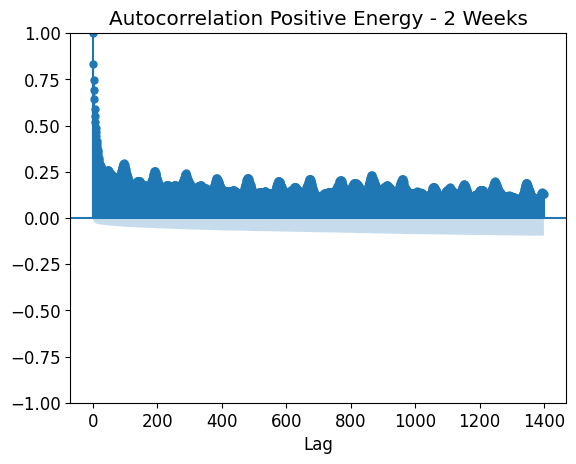
\includegraphics[width=1\linewidth]{pictures/Autocorrelation Positive Energy - 2 Weeks.png}
	\caption{Total Average Positive Energy Price}
	\label{fig:Autocorrelation Positive Energy Price}
\end{figure}

Auch Trends sind in den Daten keine vorhanden. So zeigt die Abbildung \ref{fig:posEngOverview} beispielhaft jeweils 30 Tage aus dem frühen, mittleren und spätem Jahresverlauf.
Auch hier sind weder Trends noch Saisonale entwicklungen zu erkennen.

\begin{figure}[!h]
	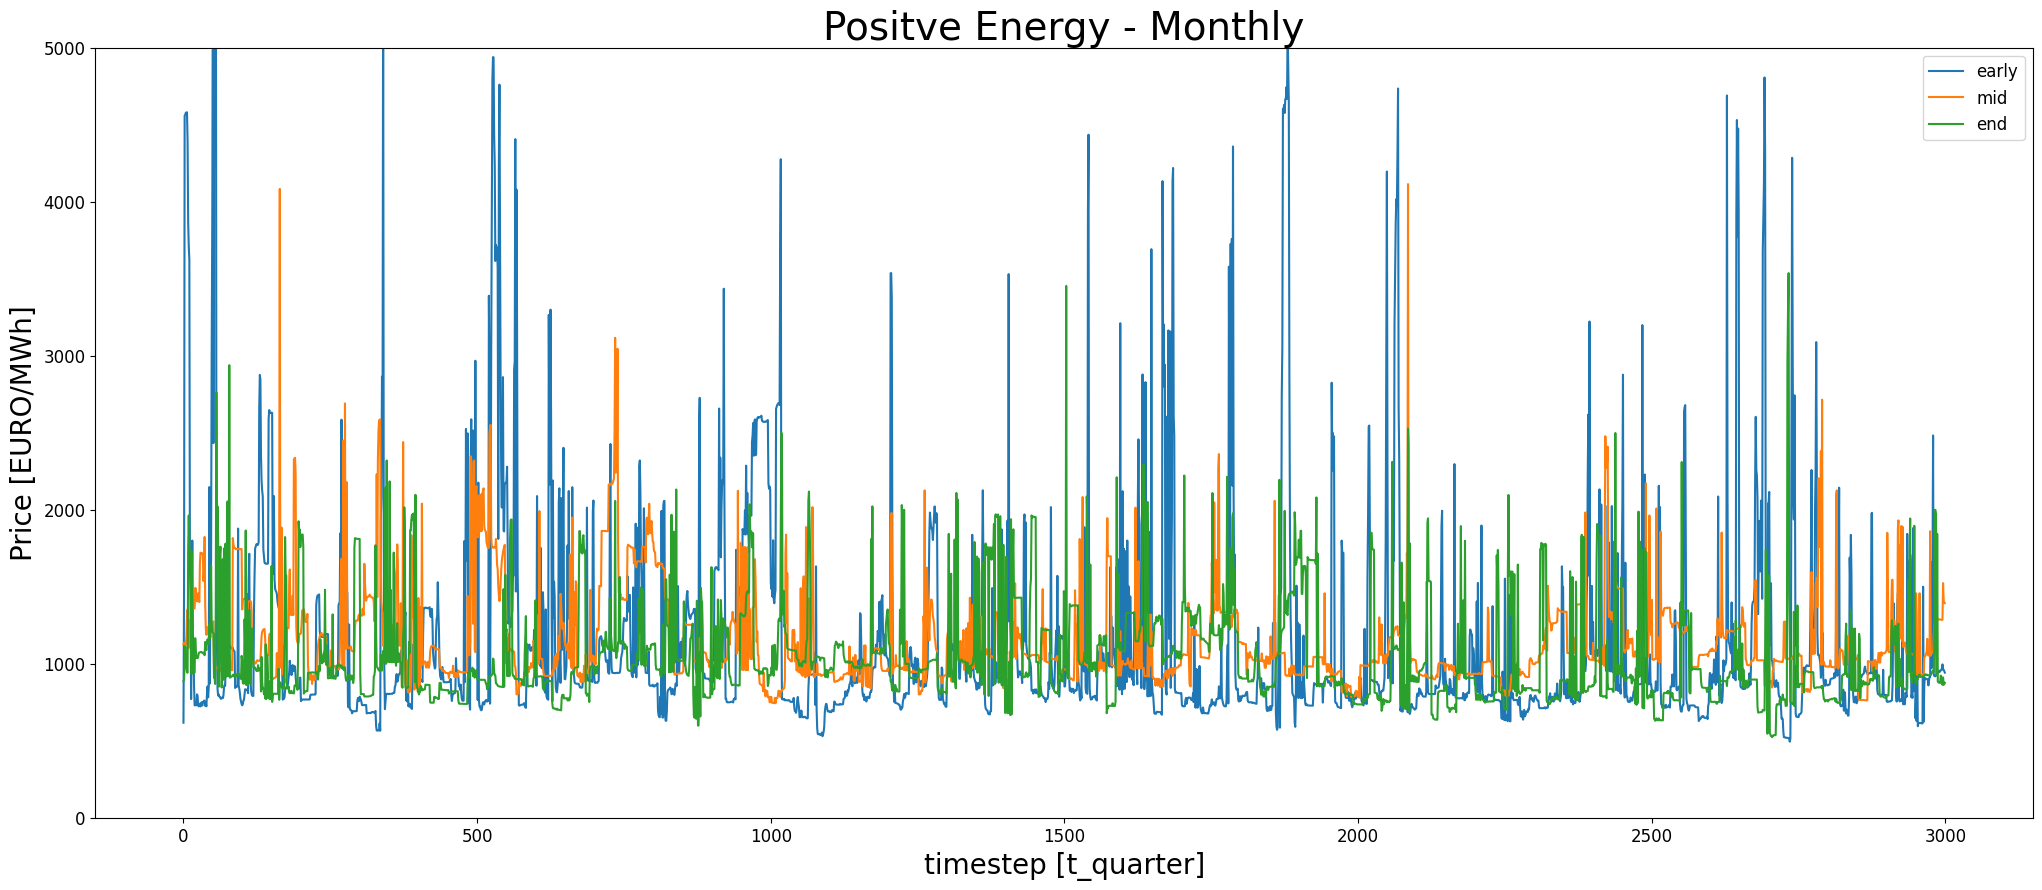
\includegraphics[width=1\linewidth]{pictures/posEngOverview.png}
	\caption{Overview Positive Energy Price}
	\label{fig:posEngOverview}
\end{figure}
\todo{das ist eine grafik mit den alten average preise, mache eine graifk mit den richtigen grenzpreisen}
\todo{grafiken verschiedene Preisszenarien}
\todo{appendix verweis zu python code}

Zu szenario generation werden Realmarkt daten aus dem Jahre 2023 herangezogen.
Das Jahr 2023 wird zuerst hinsichtlich volatiler Energiequellen untersucht [siehe Tabelle \ref{tab:energy_sources_std}].
Hierbei zeigt sich das besonders Solar und Wind Onshore Kraftwerke einer volatilen Produktion unterliegen.

\begin{table}[ht]
	\centering
	\begin{tabular}{|l|r|}
		\hline
		\textbf{Source}                 & \textbf{Standard Deviation} \\
		\hline
		Geothermal                      & 5.956190                    \\
		Fossil Oil                      & 85.360298                   \\
		Waste                           & 133.320136                  \\
		Hydro Water Reservoir           & 167.126363                  \\
		Hydro Run-of-river and poundage & 310.405850                  \\
		Biomass                         & 429.594441                  \\
		Nuclear                         & 1223.169733                 \\
		Hydro Pumped Storage            & 1543.402759                 \\
		Wind Offshore                   & 1833.588012                 \\
		Fossil Gas                      & 2916.794393                 \\
		Fossil Hard coal                & 3364.505964                 \\
		Fossil Brown coal/Lignite       & 3799.694920                 \\
		\textbf{Solar}                  & \textbf{9879.907341}        \\
		\textbf{Wind Onshore}           & \textbf{10506.831136}       \\
		\hline
	\end{tabular}
	\caption{Standard deviation per energy generator type}
	\label{tab:energy_sources_std}
\end{table}

Anschließend wird die summierte Produktion von Solar und Wind Onshore je Zeitpunkt berchnet und
durch die gesamte Produktion aller Kraftwerke zum gleichen Zeitpunkt geteilt. So erzielen wir den relativen
Anteil dieser besonders volatilen Kraftwerke an der gesamten Produktion. Die relative stündliche Produktion wurde dann verwendeten
Tagesbezogene mittelwerte zu bestimmen. Die These ist nun das wenn ein Vorhersagefehler eintritt
dieser besonders starke Auswirkungen hat wenn er an Tagen eintritt mit einem hohen Anteil volatiler produktion an der Gesamtproduktion.
Diese relativen Produktionsdaten volatiler Kraftwerke werden nun in 36 Quantile eingeteilt. Das erste, mittlere und letzte
Quantil werden nun zur Szenariogeneration benutzt.

Hierfür werden die Zeitpunkte der Quantile, die nun täglichen Daten beruhen, auf einen viertelstündlichen rythmus extrapoliert und
dazugehörigen Regelarbeitsmarkt daten vom betreffenden Zeitabschnit exportiert. Simultan dazu werden die passenden Zeitabschnitte aus
den DA und RL Zeitreihen exportiert.

So ergeben sich 10 mögliche Szenarien für Tage mit hoher, mittlerer und niedrigem Anteil einer volatilem Produktion. Die wahrscheinlichkeit
wird dabei als gleichverteilt angenommen, so das jedes Szenario die eine Wahrscheinlichkeit von 10\% hat.

Abbildung   bis
\todo{abbildungen ergänzen}
zeigt nun das zwar das allgemeine Preisniveau steigt, aber da man mit dem hohen Anteil erneuerbarer Energien
kalkuliert und somit auf die hohe volatilität eingeplant ist halten sich ansonsten die Auswirkugen in grenzen.
Die sehr hohen Ausreißer scheinen sich in den Szenarien zu zeigen in denen man nicht mit all zu hohen außreißern rechnet.
\todo{den teil drinne lassen?}



Data from ENTSOE transperency platform
\todo{ref entsoe}
-->appendix
\todo{Python Code appendix verweis}


%--> kann über  mondpreis eskapen\\
%--> können eine kaum genutzte szenarioeplosion vermeiden (wording nochmal überarbeiten)\\
%- vereinfachung der RL markt mechanik/restriktionen
%--> stellen über batterie gleichung sicher das wir immer liefer können und vermeiden so komplexe $q_RA$ restriktionen (wann wie wo gelten)\\
%--> wir stellen einfach sicher das wir immer liefern könnten und fertig\\


- verschiedene Methoden ...
-> implementiert in python
-> alle können dem model hinzugefügt werden
-> ich habe dann aus diesen und jenen gründe diese Variante gewählt
